\documentclass{article}
\PassOptionsToPackage{numbers,compress}{natbib}
\usepackage[dblblindworkshop]{neurips_2026}
\workshoptitle{Physical World AI: Geometry, Characteristics, and Multimodal Sensing}

\usepackage[utf8]{inputenc}
\usepackage[T1]{fontenc}
\usepackage{graphicx}
\usepackage{booktabs}
\usepackage{amsmath}
\usepackage{microtype}
\usepackage{xcolor}
\usepackage{url}
\usepackage{hyperref}
\hypersetup{hidelinks}
\makeatletter
\let\tablerows\@@input
\renewcommand{\@noticestring}{}
\patchcmd{\@maketitle}
  {Anonymous Author(s) \\ Affiliation \\ Address \\ \texttt{email} \\}
  {Anonymous submission \\}{}{\PackageError{paper}{Anonymous title patch failed}{}}
\makeatother

\title{MineOcclude: Separating Visual Evidence, History, and Motion Predictability}

\author{Anonymous submission}

\begin{document}
\maketitle

\begin{abstract}
Evaluating object-state representations under occlusion requires separating visual evidence, available history, and motion predictability. MineOcclude replays identical Minecraft trajectories across air, stained glass, and stone, with shared evaluation times and aligned continuous position targets. On a 25-identity graded-evidence cohort, a fixed frozen-MineWorld readout with verified RGB inputs reaches 0.083--0.107 blocks RMSE in air and glass and 1.600 under stone; a ridge baseline with the same 16-image history reaches 1.818. A variable-speed diagnostic adds 48 separate training and 48 held-out identities across two layouts and two MineWorld model sizes. At occlusion ages 1--10, 700M ridge RMSE is 1.603 blocks, compared with 1.915 for history pixels and 1.240 for a converged nonlinear probe. Removing prior images increases ridge RMSE by 2.314 blocks, but swapped-history responses do not reliably follow donor position. Direction and age remain strongly predictive at 0.154 blocks, and visible-only geometry calibration improves visible transfer without recovering hidden decoding. The protocol distinguishes input-history sensitivity, readout accuracy, and task predictability in finite-window world-model representations.
\end{abstract}

\section{Introduction}

Agents must often estimate hidden state from past observations \citep{kaelbling1998planning,hafner2019planet,zheng2026memworld}. World models can support this through learned dynamics and memory \citep{ha2018worldmodels,hafner2020dreamer,laird2025memory}. Interactive models generate visual continuations from pixels and actions \citep{micheli2023transformers,alonso2024diffusion,bruce2024genie,decart2024oasis,guo2025mineworld}, but plausible outputs do not establish which object states remain internally accessible \citep{motamed2025generative,esmati2026invisible}.

Occlusion separates current sensory evidence from prediction based on history or dynamics \citep{riochet2018intphys,weihs2022benchmarking,piloto2022intuitive,garrido2025intuitive,upadhyay2026worldbench}. Visible position can be recovered from an image \citep{chen2023beyond,zhang2026whatdo}; hidden-position estimation instead depends on prior observations or predictive cues \citep{kalman1960new,gordon1993novel,newell2025comotion,shai2024transformers}. Behavioral benchmarks assess prediction or physical plausibility \citep{yi2020clevrer,tung2023physionpp,gu2025geco}, while probes test accessible state \citep{alain2017understanding,li2023emergent,nanda2023emergent,joseph2026interpreting}. Decodability alone does not establish calibration \citep{guo2017calibration,mei2026world}, object-centric structure \citep{battaglia2016interaction,kipf2020contrastive}, or causal use \citep{hewitt2019designing,belinkov2022probing,elazar2021amnesic,geiger2024finding,alam2026causal}. We ask how accurately aligned object position remains linearly accessible as visual evidence is reduced.

MineOcclude pairs the same sheep motion, camera, and actions across visual conditions. Server state supplies wall-parallel world-$x$ targets, aligned to rendered motion with causal finite-impulse-response (FIR) filters. An earlier wall/no-wall cohort selects a spatial readout; the central study evaluates the fixed family on 25 different identities across no wall, three stained-glass materials, and an opaque wall. Verified RGB extraction and a history-matched pixel comparator first refine this study on the same central identities. A 75-identity extension tests fresh trajectories, changed geometry, and higher speed. Motivated by those comparisons, a prospectively fixed variable-speed diagnostic adds 48 training and 48 untouched test identities across two layouts, with history substitutions and a second MineWorld model size.

We make three contributions. First, a paired evidence-manipulation protocol holds realized motion and evaluation times fixed across materials. Second, a controlled evaluation procedure combines continuous aligned targets, measured image evidence, separate development data, and grouped fitting. Third, history-matched baselines, native context-length comparisons, and prospective history substitutions distinguish input-history dependence from motion predictability; nonlinear probes and visible-only calibration examine estimator and geometry dependence. Project documentation is linked through the \href{https://anonymous.4open.science/r/MineOcclude-5503/}{\textcolor{blue!70!black}{anonymous repository}}; reproduction materials are described in \autoref{app:central}.

\section{Related Work}

Learned dynamics models connect perception to planning in latent state spaces \citep{hafner2019planet,hafner2020dreamer,hafner2023mastering,schrittwieser2020muzero}. Object-centric models instead represent entities and interactions explicitly \citep{battaglia2016interaction,watters2017visual,kipf2020contrastive}. 
Benchmarks such as IntPhys, CLEVRER, PLATO, Physion, Physion++, and WorldBench evaluate object persistence, collisions, latent properties, or diagnostic physical concepts \citep{riochet2018intphys,yi2020clevrer,piloto2022intuitive,weihs2022benchmarking,tung2023physionpp,upadhyay2026worldbench, bear2021physion}. Physics-IQ and related video-model studies further show that perceptual quality and physical validity can diverge \citep{motamed2025generative,garrido2025intuitive,gu2025geco}. MineOcclude complements these benchmarks with paired occlusion and a continuous causal-FIR-aligned server-state target.

Linear probes can reveal accessible variables in intermediate representations \citep{alain2017understanding,li2023emergent,nanda2023emergent,shai2024transformers}. Recent work applies related tools to learned simulators, diffusion models, and video transformers, finding layer- and representation-dependent physical signals \citep{zhang2026whatdo,chen2023beyond,esmati2026invisible,joseph2026interpreting}. Probe results nevertheless depend on capacity, controls, and model selection \citep{hewitt2019designing,belinkov2022probing}. Removal and intervention methods ask the stronger question of whether a representation is used causally \citep{elazar2021amnesic,kim2018interpretability,geiger2024finding}.

The closest state-probing studies use different diagnostic axes. \citet{joseph2026interpreting} use layerwise probes, subspace geometry, patch-level decoding, and attention ablations to analyze physical representations in encoder-based video transformers. \citet{shin2026unobserved} use an action-conditioned visual Shell Game to test hidden-state tracking and extrapolation across swap chains. MineOcclude instead manipulates source-image evidence while holding realized trajectories and evaluation times fixed, then evaluates continuous position with condition-specific readouts in finite reset windows.



\begin{figure}[t]
\centering
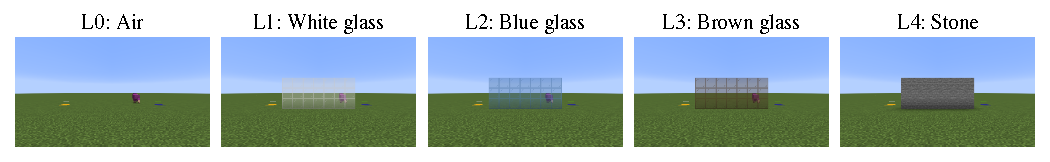
\includegraphics[width=\linewidth]{matched_captures.pdf}
\par\smallskip
{\small
\begin{tabular}{@{}ccccc@{}}
\toprule
L0: air & L1: white glass & L2: light-blue glass & L3: brown glass & L4: stone\\
$V=1$ & $V=0.8131$ & $V=0.4260$ & $V=0.1857$ & $V=0$\\
\bottomrule
\end{tabular}
\par\smallskip
Shared realized path $\longrightarrow$ common target times + aligned position labels
\par\smallskip
Separate development cohort $\longrightarrow$ fixed readout family
\par
25 central identities $\longrightarrow$ frozen RGB features $\longrightarrow$ grouped probes
}
\caption{Matched central-study captures, showing one identity at the same target time in all five conditions. Each material shares the realized trajectory and 19 evaluation times; $V$ is measured residual visual evidence. Readout selection uses separate development data. The displayed captures are recovered experimental inputs, not generated illustrations.}
\label{fig:design}
\end{figure}

\section{Methodology}
\label{sec:methodology}
\subsection{Paired cohort and evidence ladder}
\label{sec:cohort}
The central study uses 25 identities distinct from development: 13 left-to-right and 12 right-to-left paths. Each is captured in five counterbalanced conditions: air (L0), white glass (L1), light-blue glass (L2), brown glass (L3), and stone (L4). Matched captures share realized object motion, camera state, and actions. The RGB follow-up reuses these recovered captures without replacing any trajectory. The apparatus uses one layout, nominal speed 2.0 blocks/s, and process noise $q=0.05$ blocks$^2$/s at 20 Hz. Path hashes check exact pairing. \autoref{app:central} specifies the generator and calibration; \autoref{fig:design} shows matched inputs.

The 125 captures contain 22,500 source frames. Each 180-frame capture contributes 19 common target times when the full renderer-derived sheep extent would be hidden by the opaque wall. Selection is independent of material-specific decoding outcomes. The 2,375 target rows are repeated observations within 25 identities, distinct from development; no identity is replaced after outcomes are available.

The supervised target is aligned wall-parallel position, not raw same-tick server state:
\[
x_{\mathrm{align}}(t)=\sum_{k=0}^{8}h_{d,k}\,x_{\mathrm{server}}(t-k).
\]
The frozen direction-specific FIR kernels use only present and past state. They compensate for the timing difference between server updates and rendered motion, which would otherwise contribute alignment error to the decoding score. Their coefficients were inherited from earlier calibration, not fitted to central-study outcomes (\autoref{app:central}). Throughout, position error refers to this aligned target. Renderer geometry independently defines the full object extent and target times.

Residual visual evidence (RVE), $V_c$, measures noise-corrected source-image energy attributable to the sheep relative to air; $O_c=1-V_c$. Present/absent image comparisons use a shared mask, with median aggregation over blocks and nine placements (\autoref{app:central}). Stone yielded zero after noise correction and truncation, not a manually assigned endpoint. This means no positive residual energy was detected by this procedure, not that every possible cue is absent. \autoref{tab:exp3-ladder} gives the values.

RVE is an image-energy coordinate, not a visible-area fraction, an occlusion probability, or MineWorld confidence. For example, 0.186 does not mean that 18.6\% of the object is visible. The glass conditions differ in color and appearance as well as evidence magnitude. We consequently interpret the experiment as a controlled material/evidence ladder, not an isolated intervention on transparency with all other image properties fixed.

\subsection{Frozen MineWorld and feature extraction}
\label{sec:features}
MineWorld \texttt{700M\_16f} is frozen throughout \citep{guo2025mineworld}. Each target uses a teacher-forced forward, meaning that the model receives recorded images and actions, including the current recorded image, rather than an autonomous generated continuation. The 16 observations $[t-15,\ldots,t]$ span 0.75 s from first to last timestamp. Visible decoding can therefore use current sensory evidence directly.

The production extraction path calls the adapter separately for each target. Its transformer cache is refreshed before each call, and token positions start again at zero within the window. No absolute target time or oracle coordinate is supplied as a model token. Thus, this path cannot access an observation excluded from the window via a persistent cross-target cache. It is not a test of a continuously running deployed model. A current-pair feature is the final visual-token slice after processing the context, not a single-image model input. The same forward supplies layers 4, 10, and 19; storage dimensions and token offsets are in \autoref{app:central}.

The primary results below use the checkpoint's RGB convention. Source PNGs are decoded as RGB, resized by linear interpolation to $224\times384$, and normalized channelwise to $[-1,1]$. Red/blue test patches were checked at the actual tokenizer encoder input. The earlier extraction swapped red and blue, producing BGR inputs. We preserve those historical predictions and also rerun BGR on the same hardware and software as RGB, changing only that swap. This matched-runtime comparison separates channel order from the runtime change required for the new GPU.

Inference uses float16 without quantization. Frame-token caching was validated against uncached tokenization on 30 representative windows; transformer state is still reset per target. Pooling retains the original binary64 calculation. Runtime validation details are in \autoref{app:central}.

\subsection{Readout selection and grouped fitting}
\label{sec:readouts}
Separate development data selected layer-19 coarse pooling from an 11-layer global/coarse screen and a layer-19 refinement including training-only Best-K selection. The chosen family was fixed before evaluating the new cohort. Full development results, including unmet accuracy gates, remain in \autoref{app:exp2-qualification}.

The $14\times24$ visual grid is averaged into $2\times6$ cells, retaining coarse spatial organization. Flattening these pooled vectors produces 24,576 features. Layer 19 remains the primary readout; layers 4 and 10 are secondary depth checks, not candidates for reselection. We additionally fit native one-pair and eight-pair RGB inputs in air and stone, with relative positions and a fresh cache. These use the last actual recorded pairs, not repeated-image padding. Their scope was fixed from runtime measurements before inspecting the new scores.

Ridge regression gives a controlled linear readout \citep{hoerl1970ridge}. Five outer folds hold out complete trajectory identities, and four grouped inner rotations select $\alpha\in\{0.1,1,10,100,1000\}$. Standardization, hyperparameter selection, and fitting use training identities only. Holding related observations together limits dependence leakage, while inner selection separates tuning from outer evaluation \citep{roberts2017crossvalidation,varma2006bias,cawley2010overfitting,varoquaux2018crossvalidation}.

A separate probe is fitted per condition, measuring within-condition accessibility rather than transfer between materials. New RGB, BGR-replay, and baseline predictions are stored separately with the same target and fold identifiers. The primary representation is not reselected. Historical reconstruction and numerical validation are detailed in \autoref{app:central}.

\subsection{Pixel, metadata, and motion comparators}
\label{sec:baselines}
Current-pixel ridge uses $48\times28\times3$ area-resized RGB values (4,032 features); history-pixel ridge concatenates the same 16 frames available to MineWorld (64,512 features). Both use the same grouped tuning. All recorded actions are constant no-ops and are omitted after verification. Neither receives age, direction, or oracle state. History is matched, but resolution and capacity are not: MineWorld supplies pretrained nonlinear features from higher-resolution images.

The training mean is learned from outer-training targets. Direction + age fits ordinary least squares on outer-training rows to $[1,d,a,da]$, where $d=\pm1$ encodes motion direction and $a$ is context age. These privileged metadata test trajectory predictability, not equal-information competition with an image-only observer.

Last-seen holds raw server position at the last non-fully-occluded row. Constant velocity regresses the last ten pre-occlusion raw positions on time and extrapolates. Both use privileged state, are identical across an identity's conditions, and are scored against the aligned target. Oracle positions never enter neural or pixel features (\autoref{tab:baseline-inputs}).




\subsection{Metrics and inference}
\label{sec:inference}
For identity $i$ and condition $c$, let $R_{ic}$ be RMSE across the 19 held-out target rows. Tables report the mean of these identity-level errors, rather than treating all frames as independent. MAE is aggregated in the same way. Trajectory $R^2$ uses the target mean of each held-out path in its denominator; macro $R^2$ is the average of these trajectory values.

For continuity with the original study, we summarize the evidence ladder using
\begin{align}
S_i &= \operatorname{OLSslope}(R_{ic}\ \text{on}\ O_c),\\
D_{\mathrm{partial},i} &=
 \tfrac13(R_{i,\mathrm{L1}}+R_{i,\mathrm{L2}}+R_{i,\mathrm{L3}})-R_{i,\mathrm{L0}},\\
D_{\mathrm{opaque},i} &=R_{i,\mathrm{L4}}-R_{i,\mathrm{L3}}.
\end{align}
The slope summarizes the ladder; the remaining effects separate partial obstruction from the opaque increment. Condition-specific paired differences compare RGB with same-runtime BGR and history pixels; negative favors RGB. These follow-up estimates are motivated by earlier findings, not independent confirmatory tests.

Two-sided 95\% percentile intervals use 10,000 identity-bootstrap samples, seed 20260911 \citep{efron1993bootstrap}, carrying paired conditions and predictors together. They condition on fitted probes, exclude refitting uncertainty, and are not simultaneous bounds. No new significance-test family is added. The original Holm tests and bootstrap seed apply only to the reconstructed historical BGR analysis.

Age and depth summaries are descriptive. Single-age plots average absolute error; multi-age bins average within-identity RMSE. Overlapping training folds can induce dependence among held-out errors. Resampling or re-extraction does not create new identities.

The central study does not inherit the development study's nine-gate qualification rule or its 49-draw permutation test. \autoref{app:exp2-qualification} records that procedure solely as readout-development provenance.


\subsection{Prospective history and transfer tests}
\label{sec:fresh-method}
An initial extension collects 75 fresh identities across the original setting, changed geometry, and higher speed, with separate within-setting fits and unchanged-probe transfer (\autoref{app:fresh}). We then freeze a variable-speed diagnostic with 24 training and 24 test identities in each of two layouts, balanced by direction. Within each direction and split, six speeds are sampled from $[0.8,1.6]$ and six from $[2.4,3.2]$ blocks/s. All 96 identities are new and have paired air/stone captures. Four folds within the training set select ridge alpha; test identities are untouched by selection.

The primary interval is ages 1--10. Correct histories are compared with reciprocal slow/fast donor histories at the same age and with histories replaced by the repeated current image. Every intervention keeps that current image and the no-op actions fixed. Probes are trained only on correct histories. We retain the 700M final-layer coarse readout and evaluate the corresponding 300M model, plus a small nonlinear probe using training-only 64-dimensional PCA and 32 tanh hidden units. An image-only tracker estimates velocity from reliable sheep detections inside the same 16-image window. These are fixed secondary comparisons, not a new layer search.

For geometry transfer, a source probe is tested unchanged or with a shared affine output calibration fitted only on six predesignated destination-training air identities. Hidden destination labels are not used for calibration. Native destination fits provide a separate reference. New diagnostic intervals use 10,000 bootstrap draws, seed 930119, resampling identities for predictor comparisons and reciprocal donor pairs for intervention differences. Full architecture, optimizer, detector, split, and calibration specifications appear in \autoref{app:diagnostic}.

\section{Experiments}
\label{sec:experiments}
\subsection{From readout development to a new cohort}
The development study used 25 earlier trajectories to select layer-19 coarse pooling. Coarse pooling outperformed global averaging across sampled layers, and Best-K did not improve the advancing representation. Visible controls established usable position decoding, although the hidden finalist did not meet the development accuracy gates. These observations motivated evaluating the fixed family across graded visual evidence, rather than treating development as confirmation (\autoref{app:exp2-qualification}).

The central graded-visibility study fixed this family and evaluated 25 different identities. We recovered every central capture and its historical predictions, verified their hashes, and reconstructed the original statistics. The present follow-up repeats all five conditions with corrected RGB and same-runtime BGR inputs, then adds matched-history pixels and native shorter contexts. Thus the main experiment remains the graded-evidence study; corrected extraction and added comparators refine its interpretation on the same central cohort.

\subsection{Position decoding across visual evidence}
\label{sec:graded-results}
\autoref{fig:graded-results} shows the corrected-RGB results. The fixed readout recovers position in air and through all three glass materials, with RMSEs of 0.085, 0.083, 0.094, and 0.107 blocks for L0--L3. Their trajectory-macro $R^2$ values range from 0.947 to 0.973. Under stone, RMSE is 1.600 blocks, with a 95\% identity-bootstrap interval of [1.496, 1.702]. The stone identity range, 1.128--2.170 blocks, lies above the glass ranges, whose maximum is 0.197. This is a descriptive comparison across the paired identities, not an additional hypothesis test. \autoref{tab:exp3-condition} reports both pixel baselines alongside the neural readout.

\begin{figure}[t]
\centering
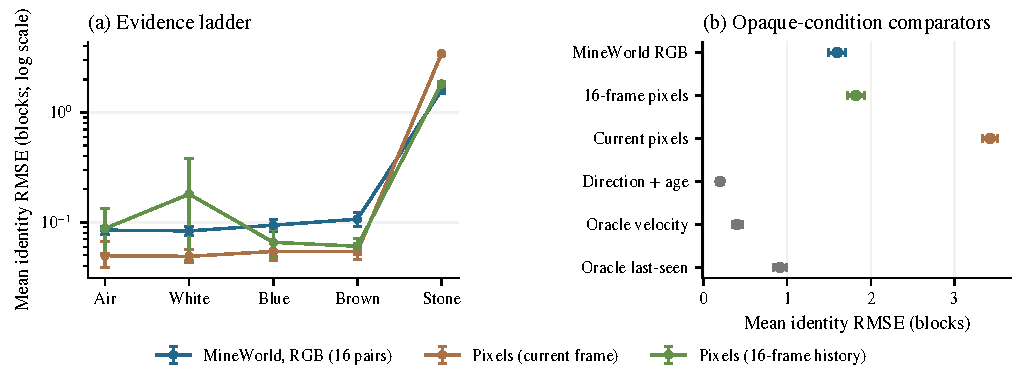
\includegraphics[width=\linewidth]{rgb_evidence_results.pdf}
\caption{Corrected-RGB evaluation of the recovered central cohort. (a) Mean identity RMSE with 95\% whole-identity bootstrap intervals; connecting lines only guide the eye between discrete materials. (b) Stone-condition comparison. The history-pixel baseline receives the same 16 images as MineWorld. Direction + age uses experiment metadata; oracle predictors use privileged state history. These inputs are not interchangeable. All intervals condition on fitted probes.}
\label{fig:graded-results}
\end{figure}

\begin{table}[!htbp]
  \caption{Corrected-RGB follow-up: mean identity performance. Errors are in blocks. All image-based predictors use the same targets and grouped folds.}
  \label{tab:exp3-condition}
  \centering
  \small
  \setlength{\tabcolsep}{5pt}
  \begin{tabular}{@{}lrrrrr@{}}
    \toprule
    Condition & MW RMSE & MW MAE & MW macro $R^2$ & Current pixels & History pixels \\
    \midrule
    \tablerows rgb_condition_rows.tex
    \bottomrule
  \end{tabular}
\end{table}
The evidence ladder contains a large opaque increment and a smaller partial-obstruction change (\autoref{tab:exp3-primary}). Moving from brown glass to stone increases mean identity error by 1.493 blocks, interval $[1.389,1.594]$. Averaging L1--L3 increases error by 0.0099 blocks relative to air, interval $[0.0021,0.0186]$. These are descriptive estimates in the RGB follow-up, not a reapplication of the historical confirmatory tests.

The slope is 1.059 blocks per unit $O_c$, interval $[0.987,1.130]$. Most of this trend is associated with the opaque endpoint. The glass results should not be interpreted as a calibrated response to transparency: materials also change color and texture, and their errors need not follow a smooth curve in the image-energy coordinate.


\subsection{Predictability and pixel comparisons}
\label{sec:baseline-results}
Current-frame pixel ridge reaches 0.049--0.054 blocks across L0--L3, below the neural errors. Under stone it reaches 3.424 blocks, matching the training-mean level. Supplying the same 16-image history reduces pixel-ridge error to 1.818 blocks. The MineWorld readout reaches 1.600, a paired advantage of 0.218 blocks, with interval $[0.173,0.265]$. The advantage over current pixels is therefore not solely an artifact of withholding all history from that comparator, although matching history substantially narrows it.

Equal history does not imply equal capacity or equal image resolution. Pixel ridge is linear in downsampled images; the neural readout is linear in pretrained nonlinear features extracted from higher-resolution images. The result supports this particular representation comparison, not superiority over all image-history estimators. In the glass conditions, history-pixel errors vary from 0.060 to 0.180 blocks, and longer input does not uniformly improve a finite-sample ridge fit. The full per-identity predictions are retained rather than selecting a favorable subset.

Metadata and oracle-history predictors assess trajectory predictability given additional information. Under stone, direction-and-age achieves RMSE 0.199399 blocks, constant velocity 0.402907, and last-seen 0.913505. Their lower errors show substantial predictability from timing, direction, and privileged pre-occlusion positions. These inputs are not supplied to the neural probe, so the ranking is not an equal-information contest. It shows why position-decoding accuracy should be interpreted alongside trajectory predictability.

In corrected RGB, stone macro $R^2=-9.324$ despite improvement over the training mean. The constant uses outer-training labels, whereas trajectory $R^2$ compares squared error with variation around each test path's own mean. For example, reducing error from 3.4 to 1.6 blocks improves on the training constant but can still be worse than the much smaller within-path variation. The test-path mean is a retrospective scoring reference, not an input supplied to the probe.

\subsection{Context age and decoder depth}
\label{sec:age}
Context age $a=1,\ldots,19$ measures 0.05--0.95 s after the last counterfactual non-fully-occluded row. The 16-pair window retains that row through $a=15$ and excludes it from $a=16$. Partial visibility does not guarantee localizable evidence. \autoref{tab:exp3-age} gives four prespecified descriptive bins; \autoref{app:central} illustrates the input-window boundary, not a measured forgetting threshold.

In corrected RGB, stone error is 0.428 and 0.369 blocks in the first two bins, then 1.938 at ages 11--15 and 2.603 at ages 16--19. Errors in the visible and glass conditions remain much lower. Thus elevated stone error begins before the last potentially informative pair is removed from the 16-pair window.


The capture geometry confirms that a 16-pair window contains $\max(16-a,0)$ rows whose counterfactual object extent was not fully occluded. Some may be only partially visible. This count establishes availability, not how well position can be localized from each frame. Age, position, and elapsed time vary together, so the curve does not identify a forgetting rate in a continuously running model.

Native one-, eight-, and sixteen-pair RGB inputs yield stone RMSEs of 3.424, 2.726, and 1.600 blocks, respectively (\autoref{fig:history}; \autoref{tab:context-lengths}). Air errors are 0.107, 0.088, and 0.085. Longer input windows therefore support better decoding in this experiment, but shortening them also changes relative positions and the fitted probe. This comparison does not isolate an internal memory mechanism.



The secondary depth panel yields a similar condition pattern at layers 4, 10, and 19 (\autoref{tab:exp3-depth}). All three support low-error decoding in L0--L3 and much larger errors in L4. These were fixed secondary probes, not additional candidates for choosing the primary result. Their common pattern does not show that the layers use the same mechanism.



\subsection{Fresh identities and history dependence}
\label{sec:fresh-results}
The initial 75-identity extension repeats the neural advantage over history pixels in the original setting and at higher speed, but not conclusively under changed geometry. Unchanged geometry transfer also degrades visible decoding, so this sensitivity is not specific to occlusion (\autoref{tab:fresh}; \autoref{app:fresh}). This motivates the separate variable-speed test, where timing and direction no longer imply a single nominal speed.

On its 48 held-out identities, correct-history stone RMSE at ages 1--10 is 1.603 blocks for 700M ridge, 1.588 for 300M ridge, and 1.915 for history pixels (\autoref{fig:diagnostic}). The pooled 700M-minus-pixel difference is -0.312, interval $[-0.784,0.013]$, so this comparison alone does not establish an advantage. Direction-and-age reaches 0.154 without commanded speed: varying speed does not eliminate trajectory predictability. Image tracking reaches 2.918, but falls back to the training mean on 59.4\% of these rows, limiting that comparator.

The nonlinear probes reach 1.199 and 1.315 under the original iteration cap. Training-limit warnings trigger a separate, fixed-configuration optimization check; all extended fits converge, reaching 1.240 and 1.341. Both budgets remain reported in \autoref{app:diagnostic}. This improves on ridge but does not remove the gap to motion metadata.

Replacing history with the current image raises 700M RMSE by 2.314 blocks, interval $[2.068,2.560]$. Swapping matched-direction histories instead changes it by -0.094, donor-pair interval $[-0.144,-0.047]$. Although the absolute prediction shift averages 2.169 blocks, its sign agrees with donor-minus-recipient position on only 32.1\% of rows. Thus input-history sensitivity is not evidence of reliable donor-position tracking. Ages 16--19 and all model responses are retained separately in \autoref{app:diagnostic}.

\begin{figure}[t]
\centering
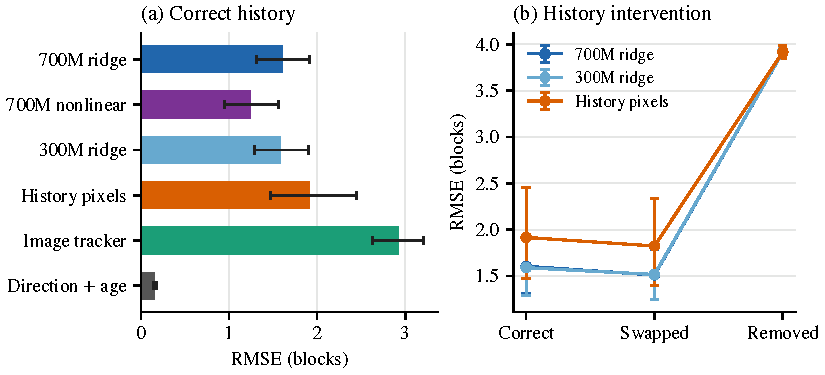
\includegraphics[width=\linewidth]{history_diagnostic_results.pdf}
\caption{Variable-speed diagnostic, 48 held-out identities at ages 1--10. (a) Correct-history performance; the nonlinear bar uses the converged optimization-check fit, while direction and age are privileged metadata. (b) History substitutions keep the current image fixed. Error bars are 95\% identity-bootstrap intervals. Paired intervention differences use reciprocal-donor-pair intervals, reported in the text.}
\label{fig:diagnostic}
\end{figure}

For the 700M probe on changed geometry, frozen-transfer air/stone errors are 1.934/2.675 blocks. Visible-only output calibration gives 0.271/3.177, compared with 0.111/1.653 after native fitting. Calibration recovers much of the visible accuracy but not hidden decoding, so a shared affine output correction is insufficient for this transfer.

\subsection{Interpretation and limitations}
\label{sec:limitations}
The material ladder separates current visual evidence from predictability; the new held-out diagnostic additionally tests sensitivity to prior images, estimator class, model size, and spatial transfer. These results concern observable position accessibility in finite reset windows, not downstream planning, calibrated uncertainty, or continuous state maintenance.

The original RGB follow-up reuses 25 central identities. Subsequent capture adds 75 exploratory extension identities and a separate prospective split of 48 training and 48 test identities. Breadth remains limited to one entity, one stochastic motion family, two layouts, and two sizes of the same pretrained model family. Fresh captures use software rendering, so historical-to-fresh differences are not attributable solely to trajectory sampling. Glass appearance changes with evidence, and geometry changes several spatial factors together.

Matching image history does not match resolution, pretraining, or total estimator capacity. The nonlinear probe is small, and the tracker uses a known-color detector with an explicit fallback when reliable observations are absent. Swapping and removing history change the input distribution and cannot alone establish an internal memory mechanism. Bootstrap intervals exclude refitting uncertainty and multiple-comparison adjustment. The prediction package makes these separate comparisons inspectable without pooling cohorts or selecting only favorable outcomes.

\section{Conclusion}
MineOcclude provides a paired protocol for separating visual evidence, history-dependent position decoding, and motion predictability. The graded-material study shows accurate RGB decoding through glass and a more demanding opaque condition. New held-out variable-speed trajectories extend the evaluation to two model sizes, nonlinear readouts, input-history substitutions, image tracking, and visible-only geometry calibration. The resulting comparisons identify estimator and input dependencies while keeping model-derived, image-based, and privileged motion predictions distinct. This supports controlled evaluation of object-position information in finite-window world-model representations.

\clearpage
\bibliographystyle{unsrtnat}
\bibliography{references}
\clearpage
\appendix
\section{Central-study measurement and implementation details}
\label{app:central}
This appendix specifies the recovered motion, alignment, input windows, measurement rules, and grouped evaluation. The original historical predictions are preserved separately from the new corrected-RGB follow-up and its same-runtime BGR replay.

\subsection{Motion, target alignment, and input window}
The lane spans $x\in[-8,8]$ at $(y,z)=(4,6)$, with a locked camera at eye position $(0.5,5.6200000048,-5.5)$, zero yaw/pitch/roll, and $70^\circ$ field of view. The wall occupies $[-3,4]\times[4,7]\times[2,3]$ in $(x,y,z)$. Minecraft 1.16.5 renders $640\times360$ frames. Conditions preserve the camera, realized motion, lighting, and action schedule; they differ in wall material.

At $\Delta t=0.05$ s, the executed update is
\[
x^{\mathrm{server}}_t=\operatorname{clip}_{[-8,8]}
 \bigl((x^{\mathrm{server}}_{t-1}+d\,2.0\,\Delta t)+\sqrt{q\Delta t}\,\epsilon_t\bigr),
\qquad \epsilon_t\sim\mathcal N(0,1),
\]
where $d$ is direction and $q=0.05$ blocks$^2$/s.

The generator uses NumPy \texttt{default\_rng(seed).standard\_normal(180)}, scaled by $\sqrt{q\Delta t}$. It accumulates drift before noise in binary64 and clamps each step. The identity seed also seeds innovations. Starting position uses the direction-specific range and \texttt{default\_rng(seed XOR 0xE3E3E3E3)}. Candidate qualification precedes outcomes; the numerical roster and start states are in the recovered manifest. All 22,500 recorded actions were checked: buttons are false, camera increments are zero, and the hotbar value is constant. They map to the same 11 action tokens in every pair. The history-pixel baseline therefore loses no variable action information by omitting constant columns.

The following raw FIR taps, ordered by lag $0,\ldots,8$, are the frozen recovered values:
\begin{center}
\small
\begin{tabular}{rcc}
\toprule
Lag & Left-to-right & Right-to-left\\
\midrule
0&0.0552210582&0.0155128136\\
1&0.0955547802&0.1420986717\\
2&0.1729033607&0.3819949723\\
3&0.2562377030&0.2529919934\\
4&0.1725945773&0.1314006058\\
5&0.1502955787&0.0092585384\\
6&0.0283805770&0.0336603539\\
7&0.0327627758&0.0330820509\\
8&0.0360495890&0.0000000000\\
\bottomrule
\end{tabular}
\end{center}
At load time, each vector is divided by its \texttt{math.fsum}; historical exact reconstruction also accumulates filtered values with \texttt{math.fsum}. The fresh extension uses the existing FIR helper's binary64 summation; its independently checked difference is below $2\times10^{-15}$ blocks. The recovery receipt reconstructs the taps from the earlier materialized stage-2 aligned labels and regenerated paths, checking 50 path hashes and 950 labels. This recovers inherited measurement calibration, not a fit to III-A decoding outcomes. The raw left-to-right vector sums to 0.9999999999 owing to decimal rounding, so normalization is part of the implementation.


\begin{center}
\small
\begin{tabular}{lll}
\toprule
Schematic target age & Recorded window relative to last non-full row $t_0$ & $t_0$ included?\\
\midrule
$a=1$ (0.05 s)&$[t_0-14,\ldots,t_0+1]$&Yes\\
$a=15$ (0.75 s)&$[t_0,\ldots,t_0+15]$&Yes\\
$a=16$ (0.80 s)&$[t_0+1,\ldots,t_0+16]$&No\\
\bottomrule
\end{tabular}
\end{center}

The timeline describes the input window, not measured forgetting. Before each target forward, the production adapter calls \texttt{refresh\_kvcache()}; positions are consecutive context-relative indices. The input preprocessing is specified in \autoref{sec:features}.

\subsection{Evidence calibration and grouped readouts}
\begin{table}[!htbp]
\caption{Central study: measured evidence ladder. $O_c=1-V_c$ is an image-energy complement, not an occlusion probability.}
\label{tab:exp3-ladder}
\centering\small
\begin{tabular}{@{}llrr@{}}
\toprule
Condition & Material & RVE $V_c$ & Complement $O_c$\\
\midrule
L0 & air/no wall & 1 & 0\\
L1 & white stained glass & 0.8131 & 0.1869\\
L2 & light-blue stained glass & 0.4260 & 0.5740\\
L3 & brown stained glass & 0.1857 & 0.8143\\
L4 & stone & 0 & 1\\
\bottomrule
\end{tabular}
\end{table}
Calibration uses two present/absent blocks (P--A--A--P and A--P--P--A), with at least eight settled frames per state per block, at nine lane positions $x=-2,-1.5,\ldots,2$, $y=4,z=6$. These are calibration placements, not the 25 experimental identities. Source values $s=v/255$ are linearized as $s/12.92$ for $s\leq0.04045$ and $((s+0.055)/1.055)^{2.4}$ otherwise. Coordinate-wise medians form each state's robust image.

For a shared mask $M$, $D=\sum_{u\in M}\|P(u)-A(u)\|_2^2$, where $P,A$ are median present/absent images. Let $N$ be the same energy between split-half absent-image medians. Excess energy is $E=\max(D-N,0)$; ratios $E_c/E_{\mathrm{L0}}$ are formed within placement and block before median aggregation. This defines $V_c$ and $O_c=1-V_c$.

For each placement, the mask threshold is the maximum squared channel-summed residual over pixels and blocks between two L0 absent-half medians. Pixels with L0 present/absent residual strictly above this threshold are unioned across blocks and dilated by a two-pixel square neighborhood. This one mask is shared across materials. Absent frames are split by ascending capture index into equal first/last halves; an odd middle frame is omitted. Ratios of nonnegative excess energies are formed within block and placement before taking the median over the two blocks and then over the nine placements. The calibration minimum is a protocol requirement; the exact realized image inventory is needed to inspect individual captures.

Each pair contains 336 visual and 11 action tokens. A 16-pair sequence has 5,552 tokens and hidden width 2,048. Its current visual offsets are $[5205{:}5541)$; action tokens are excluded from readout vectors. The recovered historical extraction stored 750 float16 arrays of shape $[19,336,2048]$, approximately 18.26 GiB together. The follow-up instead stores pooled $[19,24576]$ binary64 arrays. Hooks at layers 4, 10, and 19 share a forward. Input-token caching is frame-local and does not cache temporal transformer state.

Outer folds sort identities by (seed, identity ID) within direction and allocate five identities per fold with left/right counts $(3,2),(2,3),(3,2),(2,3),(3,2)$. Four deterministic inner rotations are constructed inside each outer training set. Exact membership is bound by the cohort/fold manifests; every condition and row of an identity stays together. All training-dependent transforms and ridge selection remain inside these splits.

\subsection{Input convention and matched-runtime comparison}
\label{sec:temporal}
The original BGR predictions remain useful as an audit trail, but they are not relabeled as corrected inputs. A direct historical-to-new comparison would also change the GPU and PyTorch runtime. We therefore repeat BGR extraction on the RGB runtime with the same checkpoint, precision, frames, actions, pooling, and folds. The only preprocessing difference in that pair of runs is the red/blue channel swap. \autoref{tab:channel-order} reports all three configurations separately.

Under stone, the same-runtime BGR replay gives 1.693 blocks RMSE versus 1.600 for RGB, a paired reduction of 0.093 blocks, interval $[0.040,0.153]$. The channel-order effect is not uniform: RGB reduces white-glass error by 0.014 blocks but increases brown-glass error by 0.021. The historical BGR value of 1.645 is distinct from the new replay. The table therefore distinguishes historical results from the controlled preprocessing comparison.

\begin{table}[!htbp]
\caption{Predictors receive different information. Server-state targets supervise fitting and scoring but never enter the neural or pixel feature vectors.}
\label{tab:baseline-inputs}
\centering\small
\begin{tabular}{@{}p{0.27\linewidth}p{0.65\linewidth}@{}}
\toprule
Predictor & Information supplied\\
\midrule
MineWorld current & Recorded visual/action window and pretrained context-dependent features\\
Pixel ridge & One downsampled source RGB image\\
History-pixel ridge & The same 16 source RGB images as MineWorld, in time order\\
Direction + age & Experiment metadata: direction and counterfactual occlusion age\\
Last-seen & Privileged raw server position at the last non-fully-occluded row\\
Constant velocity & Ten privileged pre-occlusion raw server positions\\
Training mean & Outer-training labels only\\
\bottomrule
\end{tabular}
\end{table}
\begin{table}[!htbp]
  \caption{Corrected RGB: descriptive mean identity RMSE by context-age bin (blocks).}
  \label{tab:exp3-age}
  \centering
  \small
  \begin{tabular}{@{}lrrrrr@{}}
    \toprule
    Age & L0 & L1 & L2 & L3 & L4 \\
    \midrule
    \tablerows rgb_age_rows.tex
    \bottomrule
  \end{tabular}
\end{table}
\begin{figure}[t]
\centering
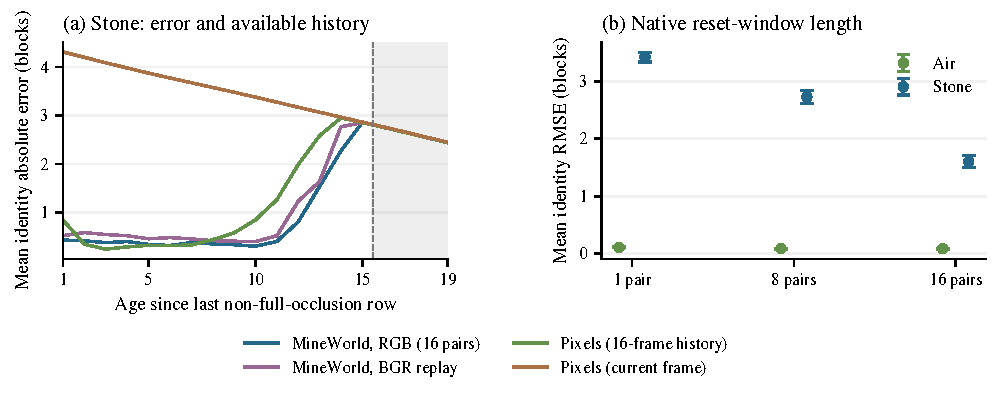
\includegraphics[width=\linewidth]{rgb_history_results.pdf}
\caption{History diagnostics. (a) Mean identity absolute error at each age; one row per identity makes this MAE rather than multi-row RMSE. Shading starts when the last non-fully-occluded observation leaves the input at age 16. (b) Separately fitted native-context RGB probes, with 95\% identity-bootstrap intervals. Context length changes history and relative positions, not an identified memory circuit.}
\label{fig:history}
\end{figure}
\subsection{Additional central results and access}
\begin{table}[!htbp]
  \caption{RGB evidence-ladder estimates. Two-sided 95\% paired identity-bootstrap intervals are descriptive, not simultaneous confidence bounds. Units are blocks for $D$ and blocks per unit evidence complement for $S$.}
  \label{tab:exp3-primary}
  \centering
  \small
  \setlength{\tabcolsep}{3.5pt}
  \begin{tabular}{@{}lrr@{}}
    \toprule
    Estimand & Mean & 95\% identity-bootstrap CI \\
    \midrule
    $S$ & $1.059$ & $[0.987,1.130]$ \\
    $D_{\mathrm{partial}}$ & $0.0099$ & $[0.0021,0.0186]$ \\
    $D_{\mathrm{opaque}}$ & $1.493$ & $[1.389,1.594]$ \\
    \bottomrule
  \end{tabular}
\end{table}

To evaluate another checkpoint, a researcher would keep the paired captures, aligned targets, and identity splits fixed, select the readout on separate development data, and submit held-out predictions indexed by identity, condition, target time, and predictor. Reporting both image-based and metadata/oracle comparisons then separates position accessibility from trajectory predictability. The prospective diagnostic in \autoref{app:diagnostic} implements this comparison for a second MineWorld model size while keeping its family and input convention fixed.

\begin{table}[!htbp]
  \caption{Corrected RGB: mean identity RMSE across the fixed depth panel (blocks).}
  \label{tab:exp3-depth}
  \centering
  \small
  \begin{tabular}{@{}lrrrrr@{}}
    \toprule
    Layer & L0 & L1 & L2 & L3 & L4 \\
    \midrule
    \tablerows rgb_depth_rows.tex
    \bottomrule
  \end{tabular}
\end{table}
The original capture and extraction stages took 2,975.5 s and 4,730.8 s, respectively. Recovered receipts identify an NVIDIA L4 with PyTorch 2.6.0/CUDA 12.6 for historical extraction. The follow-up uses one RTX 5090 (32 GB), a Ryzen 9 9950X3D, 64 GB installed host RAM, and a dedicated WSL Python 3.10.21 environment with PyTorch 2.7.1/CUDA 12.8, NumPy 1.26.4, and float16 inference. The full dependency snapshot accompanies the code. These environments differ; only the new RGB/BGR pair controls that difference.

Full RGB and BGR extraction each processes 2,375 targets, taking 504.8 s and 515.3 s after model loading. The 950-target native one- and eight-pair runs take 90.4 s and 137.9 s. Summed fitting time for the 44 new predictor/condition fits is 79.7 s, with CPU fitting overlapping extraction. Production dispatch through final extraction takes 22.7 min including model loads and BGR validation. Peak allocated tensor memory during profiling is 4.45 GiB, excluding display/driver allocations and allocator reservations. Artifact recovery, environment setup, downloads, and initial validation take approximately 37 min separately; manuscript preparation is not counted as GPU compute. These are measured follow-up costs, not a total-project compute claim.

Actual encoder red/blue patch inputs, normalization, dimensions, and interpolation were checked against the reference path. The 30-window validation spans both directions, all five conditions, and early/late ages. Cached and uncached frame tokens matched exactly, as did repeated fresh-cache forwards. Replacing the action tokens following the current visual slice left all three readouts unchanged. Every complete input window was checked against its capture and target indices. Frame-token caching does not carry observations across independent transformer calls.

The complete 125-capture corpus was recovered from five hash-verified archives. All 24,500 files, including 22,500 PNGs, matched their recorded checksums. All 2,375 aligned targets were reconstructed from the recorded coordinates and frozen FIR taps with maximum absolute error zero. The original 4,833,894-byte prediction package passed its raw-file hash and canonical seal; these are distinct checksums. Its 23,750 cells have complete unique identity/condition/row/model keys. Recomputing the original primary means, standard errors, p-values, adjusted p-values, and bootstrap intervals reproduced the recorded values exactly.

The follow-up snapshot includes every new held-out prediction, target, exact fold, selected alpha, feature hash, input configuration, source script, and bootstrap setting. Five genuinely matched central captures supply \autoref{fig:design}. Running \texttt{python scripts/rgb\_replication/reproduce.py} from the extracted snapshot verifies file hashes, rebuilds the statistics, checks equality with the supplied numerical summary, and regenerates figure and table files without a GPU. Full inference additionally requires the verified captures and upstream checkpoint; weights are not redistributed in the compact snapshot. Anonymous public distribution of the new package has not yet been verified.

The optimized ridge implementation was compared with the unmodified reference on this machine. Predictions matched exactly for all five current-pixel and history-pixel conditions and the neural air/stone checks. All 125 regenerated current-pixel feature hashes matched the original feature index. Nevertheless, cross-host pixel refitting was not bitwise identical, with maximum per-row discrepancy 0.049 blocks. Near-constant image columns and floating-point linear algebra can affect fitting and alpha selection. The new baselines therefore use the new runtime consistently, while the original sealed predictions remain the basis for historical reconstruction. Rebuilding statistics from stored predictions does not require reproducing those fitting differences.

\begin{table}[!htbp]
\caption{Layer-19 mean identity RMSE and channel-order differences (blocks). BGR replay and RGB use the same runtime; historical BGR uses the original L4 runtime. A negative difference favors RGB.}
\label{tab:channel-order}
\centering\small
\begin{tabular}{@{}lrrrrl@{}}
\toprule
Condition & Historical BGR & BGR replay & RGB & RGB minus replay & 95\% paired CI\\
\midrule
\tablerows rgb_channel_rows.tex
\bottomrule
\end{tabular}
\end{table}

\begin{table}[!htbp]
\caption{Native shorter-context RGB probes. Each context length has a separately fitted grouped probe; the primary remains the 16-pair layer-19 readout.}
\label{tab:context-lengths}
\centering\small
\begin{tabular}{@{}lrrrr@{}}
\toprule
Context pairs & Air RMSE & Air 95\% CI & Stone RMSE & Stone 95\% CI\\
\midrule
\tablerows rgb_context_rows.tex
\bottomrule
\end{tabular}
\end{table}

The historical secondary temporal analyses remain available in the recovered package. Current-minus-previous features reduced performance by 0.375919 blocks when averaged over L1--L4; previous/current concatenation changed the mean by 0.000060 blocks. These concern the historical BGR representation, not the new RGB context-length comparison. They are not substituted into the corrected results.


\begin{table}[!htbp]
\caption{Fresh cohorts, 25 identities each. Mean identity RMSE in blocks after within-setting refitting. The last columns give neural minus history-pixel stone RMSE and its paired 95\% bootstrap interval; negative favors the neural readout.}
\label{tab:fresh}
\centering\small
\setlength{\tabcolsep}{4pt}
\begin{tabular}{@{}lrrrrl@{}}
\toprule
Setting & MW air & MW stone & History stone & Difference & 95\% CI\\
\midrule
\tablerows fresh_rows.tex
\bottomrule
\end{tabular}
\end{table}
\section{Fresh-cohort capture and generalization details}
\label{app:fresh}
The extension's roster and primary analysis were fixed before neural or pixel decoding outcomes were inspected. It contains 75 new deterministic seeds, disjoint from seeds in historical repository records and from six engineering-pilot identities. Each setting has 13 left-to-right and 12 right-to-left paths. Starts are sampled uniformly at magnitudes 7.3--7.9 blocks on the corresponding side of the lane. The same drift-plus-noise generator uses $q=0.05$, $\Delta t=0.05$ s, and 180 frames. Candidates must provide 19 consecutive counterfactual fully occluded rows after at least 16 input frames, no lane-boundary clamp on target rows, and aligned target standard deviation above 0.10 blocks. These geometry/target-spread checks precede readout outcomes; the roster retains candidate rejections. No failed or unfavorable decoding result is replaced.

The original arrangement has sheep depth $z=6$ and wall depth $[2,3]$. The geometry extension moves the sheep to $z=8$ and wall to $[3,4]$, retaining the same wall-parallel lane and locked eye position $(0.5,5.6200000048,-5.5)$. Thus it changes apparent object scale and occluding geometry together. The speed extension retains the original arrangement but raises drift magnitude from 2.0 to 3.0 blocks/s. All conditions use air or stone; the central glass calibration values are not assigned to these new scenes.

\begin{figure}[!htbp]
\centering
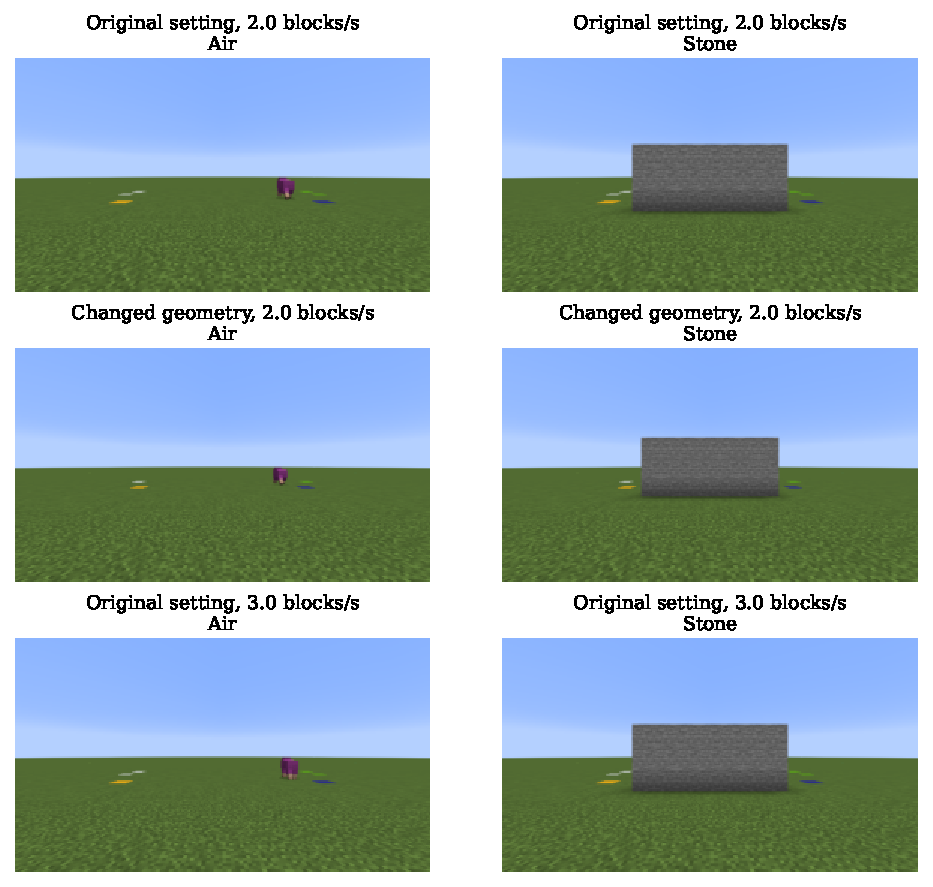
\includegraphics[width=.82\linewidth]{fresh_captures.pdf}
\caption{Actual fresh-cohort recordings. Each row shows one identity's air/stone pair at its first selected target time. The same state and time are used within each pair; different rows are different identities and need not have equal position. These are captured Minecraft inputs, not model generations.}
\label{fig:fresh-captures}
\end{figure}

An isolated Minecraft 1.16.5/Fabric runtime runs under Xvfb with Mesa llvmpipe software rendering. The original capture mod is rebuilt without source edits. Twelve disjoint engineering captures cover both directions in all three settings and both materials. Mandatory present/absent/present liveness checks, physical receipts, drained writers, exact tick/frame/action joins, image dimensions, camera state, and target identity are verified. Production validation independently regenerates every path and target, checks exact air/stone pairing, and checks the magenta sheep is visible in air and absent in all opaque target images. This pixel check validates the selected geometry; it does not shift target times or replace labels.

The historical direction-specific FIR target definition is retained, not recalibrated on decoding outcomes. On visible pilot images, projected silhouette motion is checked against these labels with centered RMSE below 0.15 blocks and median offset magnitude below 0.30 blocks. Silhouette centers include view-dependent wool geometry, so this is an engineering motion-alignment diagnostic rather than an exact measurement of the rendered entity origin. The observed offsets are not used to modify labels. The admission receipt records this limitation and all pilot checks.

Within each setting, successive admitted identity indices are assigned to five outer folds modulo five. Each condition of an identity stays in the same fold. Four remaining groups provide inner rotations. All 150 captures contribute 19 rows, yielding 2,850 targets and 19,950 primary prediction cells across seven predictors. The source-only transfer analysis uses all 25 fresh original-setting identities after five-fold source-only alpha selection and evaluates 50 destination identities. Its 5,700 cells are kept separately. Destination labels are not used for scaling, fitting, or alpha selection.

Transfer removes exactly constant source-training columns before scaling, including inside each source-validation fold, and freezes that mask for destination prediction. This source-only safeguard was specified before outcomes to avoid spurious weights from round-off in repeated pixel values. The primary within-setting fits retain the historical-compatible implementation. Transfer is consequently a separately documented estimator, not an exact reuse of an outer-fold fit from the primary table.

Higher speed also changes the distance traveled within the fixed 19-age evaluation window and its target spread. The resulting setting-specific errors are not an isolated causal estimate of forgetting rate. Within each air/stone pair, positions and evaluation times remain exactly matched.

\begin{table}[!htbp]
\caption{Fresh-cohort comparator RMSE after within-setting fitting (blocks). Motion predictors use privileged state or metadata, not the same information as image-based methods.}
\centering\small
\begin{tabular}{@{}llrrrr@{}}
\toprule
Setting & Material & Current pixels & Direction/age & Last-seen & Constant velocity\\
\midrule
\tablerows fresh_baselines_rows.tex
\bottomrule
\end{tabular}
\end{table}

\begin{table}[!htbp]
\caption{Secondary unchanged-probe transfer RMSE (blocks). Scalers, alpha selection, and probe fitting use only the fresh original-setting cohort. These are not within-setting cross-validation estimates.}
\centering\small
\begin{tabular}{@{}llrrr@{}}
\toprule
Destination & Material & MineWorld & Current pixels & History pixels\\
\midrule
\tablerows fresh_transfer_rows.tex
\bottomrule
\end{tabular}
\end{table}

Raw server position, rather than the aligned target series, supplies last-seen and constant-velocity inputs. This wording follows the actual historical loader and the fresh implementation; an earlier baseline module docstring called these inputs aligned. The supervised/scored target remains the direction-specific FIR quantity in every condition. This documentation correction does not change historical numerical results.

The compact extension package contains all primary and transfer predictions, exact targets and folds, capture hashes, the frozen protocols, engineering receipts, and CPU-only rebuilding scripts. Hash verification and reconstruction of every reported summary are performed independently of feature extraction. Full refitting additionally needs the captured images and checkpoint; the compact package does not redistribute Minecraft binaries or model weights. Anonymous public distribution still requires a separate release and access check.

On the same RTX 5090 workstation, fresh production capture took 57.47 minutes including runtime startup. RGB extraction processed 2,850 targets plus validation calls in 10.12 minutes including model loading. Pixel features took 111.87 seconds, overlapping neural extraction. Primary and transfer fits, including reference checks, used 93.88 and 4.10 summed seconds, respectively. Peak allocated GPU tensor memory was 4.45 GiB and peak reserved memory was 6.59 GiB. Runtime installation, engineering pilots, manuscript work, and packaging are additional costs. The unmodified capture mod passed all 43 Java tests. Selected Python tests yielded 154 passes and one historical bitwise FIR assertion discrepancy; an independent summation check bounded label differences below $2\times10^{-15}$ blocks. The fresh statistics passed six dedicated tests and a clean NumPy-only reconstruction of all 25,650 prediction cells.

\section{Readout-development provenance}
\label{app:additional-detail}
\label{app:exp2-qualification}
The earlier paired study (Experiment II in the execution records) selected the representation subsequently fixed for the central graded-visibility study (Experiment III-A). It reused 25 trajectories and sampled layers $\{0,2,4,6,8,10,12,14,16,18,19\}$ with global mean and coarse $2\times6$ pooling. Layer-19 refinement compared global, coarse, and Best-K readouts, with $K\in\{1,4,16,64\}$ selected using training identities only. Its nine-gate decision below is not the decision rule for the new-cohort study.

The paired \texttt{NO\_WALL} and \texttt{WALL\_HIDDEN} populations each contained 475 rows, or 19 per identity. The separate \texttt{WALL\_VISIBLE} control contained 846 rows from a different row and target-range population. It tested visible-position decoding in the wall domain, rather than serving as a matched effect-size comparison with the paired populations.

\begin{table}[!htbp]
\caption{Earlier-study qualification. Stability thresholds apply to group means of $\Delta_A$, in blocks. The follow-up uses the estimates in \autoref{sec:inference}, not this ledger.}
\label{tab:gates}
\centering
\small
\begin{tabular}{clc}
\toprule
Gate & Earlier-study requirement & Finalist\\
\midrule
G1 & Provenance, cohort, target, implementation, and leakage checks & Pass\\
G2 & Mean $\Delta_A>0$ and bootstrap lower bound $>0$ & Pass\\
G3 & Macro $R^2>0$ and bootstrap lower bound $>0$ & Not met\\
G4 & RMSE $\leq0.50$ blocks & Not met\\
G5 & $\geq4/5$ fold means $>0$; every fold mean $>-0.10$ & Pass\\
G6 & Both direction means $>0$ & Pass\\
G7 & $\geq4/5$ phase means $\geq0$; every phase mean $>-0.10$ & Pass\\
G8 & Both visible controls qualify & Pass\\
G9 & Selection-aware $p_A\leq0.05$ & Pass\\
\bottomrule
\end{tabular}
\end{table}

For identity $i$, $\Delta_{A,i}$ is training-mean RMSE minus probe RMSE. The five fold means were $0.38572$, $0.42825$, $0.44047$, $0.38606$, and $0.35533$. Direction means were $0.37864$ and $0.42141$; the available record does not identify their displayed left/right order. Phase means for phases $0,3,6,9,12$ were $1.04799$, $0.64187$, $0.30272$, $-0.00659$, and $0.00985$. These values establish G5--G7 without introducing new thresholds.

The final three-candidate refinement selected layer-19 coarse pooling with mean $\Delta_A=0.3991669$. Each of 49 null draws permuted hidden activation blocks within direction-by-phase groups and reran the reported selection procedure, leaving targets, folds, baselines, age, and visible controls fixed \citep{ojala2010permutation}. The null mean was $0.3845741$ and its maximum $0.3989598$, only $0.0002071$ blocks below the observation. The add-one p-value was $(1+0)/(49+1)=0.02$, its minimum resolution \citep{phipson2010permutation}. The finalist's macro $R^2=-13.8263$ and RMSE $2.0711$ nevertheless failed G3 and G4. The summary identifies three layer-19 refinement candidates but does not establish that the earlier 22-cell layer screen was rerun for each null. We therefore do not claim adjustment for that entire earlier search. These statistics concern development only, not the central three-effect tests.

Extraction for that study involved 1,796 target rows and 11 tensors per forward, giving 19,756 arrays of shape $[336,2048]$ in little-endian float16. The tensor payload totaled 27,189,313,536 bytes (25.32 GiB). The project describes extraction code, configurations, inventories, and integrity manifests separately from this raw corpus. Complete raw-data access and an executable public snapshot still require verification; hashes alone do not establish reproducibility.

The earlier source audit checked model identities, target alignment, tensor integrity, selected features, folds, and the decisive screening/refinement metrics. It did not independently recompute the final selection null, bootstrap intervals, visible-control statistics, or all gate arithmetic. These results provide readout-development provenance rather than independent confirmation of every reported statistic.

The historical development and central studies used the legacy BGR convention. The new RGB follow-up changes the input convention but keeps the selected layer-19 coarse family fixed. Development was not rerun to choose a different layer under RGB. The runtime checks in \autoref{sec:features} establish the new input channel order directly.


\clearpage
\section{Prospective variable-speed history diagnostic}
\label{app:diagnostic}

\subsection{Question, capture design, and split}
The earlier constant-speed cohorts leave substantial predictability in direction and occlusion age. We therefore freeze a new diagnostic before inspecting test predictions. It retains the original stochastic motion generator, sheep, camera, RGB preprocessing, and 16-pair reset window, but varies nominal speed between identities within each layout and direction. Six speeds per direction are sampled uniformly from $[0.8,1.6]$ and six from $[2.4,3.2]$ blocks/s. Start magnitudes are sampled uniformly from $[7.3,7.9]$, on opposite sides for the two directions. Process noise remains $q=0.05$ at $\Delta t=0.05$ s. No unobserved event independently changes velocity during occlusion.

Each of layouts 01 and 04 has 24 training and 24 untouched test identities, balanced by direction and speed band. All 96 seeds are disjoint from historical records, the previous 75-identity extension, and engineering pilots. Every identity has paired air and stone recordings of 180 frames. The first 19 consecutive fully occluded times are selected by geometry, with at least 16 preceding/current frames available and no target clamp. The resulting 192 recordings supply 34,560 source frames and 3,648 paired-condition target rows. These rows are repeated measurements, not independent samples. Sixteen separate pilot recordings, covering both speed endpoints, directions, and layouts, check capture and alignment but never enter scientific fitting or scoring.

Physical receipts, paired path hashes, camera/target identity, writer completion, action constancy, exact frame/tick joins, and target-image checks are required before extraction. The inherited direction-specific FIR target is retained, with pilot silhouette checks as an engineering diagnostic rather than a newly fitted target. Every new capture uses the same fixed software-rendering configuration. The protocol, roster, analysis specification, and source hashes are preserved before test scoring. This study is a prospective test of a previously chosen readout family on new identities, not an independent research-group replication.

One test path briefly becomes fully occluded at frame 39, reappears at frames 40--41, and begins its selected consecutive segment at frame 42. It is retained under the original selection rule. The validation initially assumed all frames before the consecutive segment were non-fully-occluded; this shortcut was replaced with exact recorded-visibility counts. The original failed check and correction record are preserved. No capture, target, feature, prediction, statistic, or inclusion decision changes. The zero-prior-visibility control at ages 16--19 still holds for every identity.

\subsection{History interventions and model sizes}
For each test identity, a reciprocal slow/fast donor is fixed within the same layout and direction. Rank $j$ is paired with $(j+6)\bmod 12$. The correct condition uses the recipient's recorded 16 images. The swapped condition takes the donor's preceding 15 stone frames at the same occlusion age and appends the recipient's original current frame. The removed condition repeats that current stone frame 16 times. Action tokens are constant and remain unchanged. Models are fitted only on correct training histories, with no fitting on intervened test inputs.

The primary interval is ages 1--10. Ages 11--15 are secondary, and ages 16--19 form a control where the last geometry-defined non-fully-occluded observation has left the reset window. We record the number of such observations, current-frame donor/recipient pixel differences, and tracker detection coverage. Full geometric occlusion alone does not prove absence of every indirect image cue. Repeated-image removal changes the input distribution, while a donor swap changes prior images rather than an identified internal representation. These tests establish input-history dependence to the extent supported by their results, not a causal circuit or persistent memory outside the window.

The primary model remains \texttt{700M\_16f}. A secondary \texttt{300M\_16f} checkpoint uses the same official model family, shared tokenizer, 20 decoder layers, and final-layer $2\times6$ pooling. Its hidden width is 1,024 rather than 2,048, yielding 12,288 rather than 24,576 pooled features. Both checkpoints are hash-pinned, safely loaded with every inference parameter present, and evaluated in float16 with RGB patches checked at the tokenizer encoder input. This comparison extends parameter scale within one model family, not architecture or pretraining diversity.

\subsection{Training-only model fitting and comparators}
For each layout and material, four identity-grouped folds within the 24 training identities select hyperparameters. Fold membership is fixed by rank modulo four, with 18 fit and six validation identities per rotation. The objective is mean identity RMSE over all 19 training targets. The selected model is refitted on all 24 training identities before prediction on the 24 disjoint test identities. Ridge uses $\alpha\in\{0.1,1,10,100,1000\}$. Feature columns constant in training are removed, and means and scales are fitted on training rows only.

The secondary nonlinear probe uses a training-only 64-component PCA, or fewer components if the training matrix has lower available dimension, followed by 32 tanh hidden units and a scalar output. L-BFGS uses at most 500 iterations, 25,000 function evaluations, and tolerance $10^{-5}$. Training-only target standardization is applied. Penalties $\{0.001,0.1\}$ are selected by the same four folds; predictions average seeds 1301, 1302, and 1303. PCA seed 93011 is fixed. Optimizer warnings are retained in the fit records. The test set does not select a layer, pooling rule, penalty, or seed.

All original nonlinear training searches reported iteration-limit warnings. Before consulting their test scores, a separate optimization check was frozen: refit the already selected configurations with limits of 10,000 iterations and 250,000 function evaluations, leaving penalties, architecture, PCA, seeds, and data assignments unchanged. This check is additional to the original prospective protocol and does not reopen hyperparameter selection. All 24 final seed-level refits converge without warnings, in 774--4,081 iterations. Both budgets and their 7,296 additional prediction cells are retained; the larger budget is not selected according to test performance.

Current-pixel and 16-image history-pixel ridge retain the original $48\times28$ RGB features. An additional image-only tracker uses the largest connected component satisfying $R>45$, $B>30$, $R>1.4G$, and $B>1.25G$. A linear mapping from component horizontal center to aligned world position is fitted only on training air frames with index at least 15 and absolute raw position below six blocks. The median training component width, height, and area set a fixed reliability rule: at least 0.85 of median width and height and 0.65 of median area. At test time, the last at most ten reliable detections inside the same 16-frame image window are extrapolated by ordinary least squares in time. One detection uses last position; no detection uses the training target mean. The tracker receives no test state, direction, speed, or geometry-defined visibility. Its fixed magenta detector exploits the known sheep appearance and is not a general-purpose tracker.

Direction-and-age, training mean, oracle last-seen position, and oracle constant velocity retain their previous definitions. The oracles use privileged raw pre-occlusion state and are not constrained to the 16-image window. Their information differs from the image-based estimators and is labeled separately. None of the image-based predictors receives commanded speed. The nonlinear probe relaxes the linear-readout restriction but does not match MineWorld's image resolution, pretraining, or total estimator capacity to pixel ridge.

\subsection{Visible-only calibration and inference}
For geometry transfer, source-layout probes are fitted on the 24 layout-01 training identities. They are evaluated unchanged on the 24 layout-04 test identities. A separate calibration uses only the six layout-04 training identities with ranks $\{0,4,8\}$ in each direction, and only their air observations. We fit an intercept and slope from the source air probe's predictions to these air targets, then apply the identical output mapping to the source air and stone probes. Destination hidden labels never enter that calibration. Frozen transfer, visible-calibrated transfer, and native within-layout fitting are all reported; none is selected using test scores.

We report mean identity RMSE, MAE, and trajectory-macro $R^2$ by layout and pooled over the balanced test set. The primary ages 1--10, secondary ages 11--15, terminal ages 16--19, and full 19-row summary are retained. Intervals use 10,000 paired bootstrap draws with seed 930119. Ordinary predictor comparisons resample identities; history-intervention comparisons resample reciprocal donor pairs because recipients share donor data. Intervals condition on the fitted models and are not simultaneous bounds. Swapped-history response includes absolute prediction change, agreement of its sign with donor-minus-recipient target position, and errors relative to both targets. These estimates describe the fixed diagnostic rather than reopening the earlier development search.

\begin{figure}[!htbp]
\centering
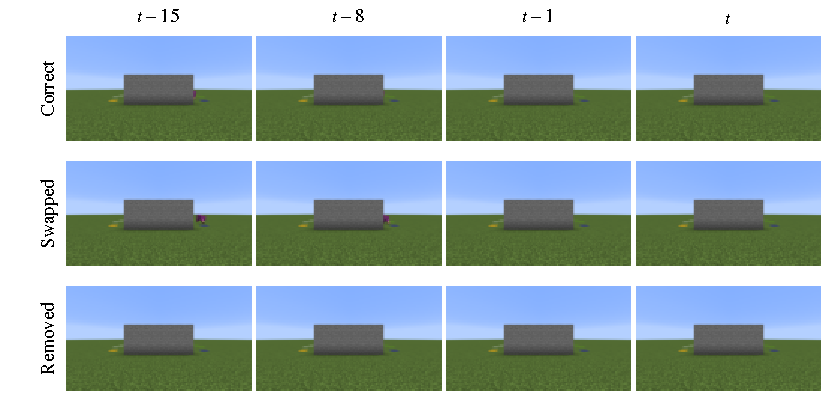
\includegraphics[width=\linewidth]{history_intervention_inputs.pdf}
\caption{Actual image-history substitutions for the first predetermined original-layout, left-to-right slow test identity at age 1. Four of the 16 input times are displayed. The swapped row uses its preassigned fast donor for earlier images and the recipient for the current image. The removed row repeats the recipient current image. Images are recorded inputs, not generated illustrations or outcomes selected for visual effect.}
\label{fig:history-inputs}
\end{figure}
\begin{table}[!htbp]\centering\small
\caption{Pooled test identities: mean identity RMSE in blocks. Air is summarized over ages 1--10. Stone columns retain the prespecified age bins. Each layout has 24 test identities; the pooled table has 48.}
\begin{tabular}{@{}lrrrrr@{}}\toprule Predictor & Air 1--10 & Stone 1--10 & 11--15 & 16--19 & Stone 1--19\\\midrule
700M ridge & 0.110 & 1.603 & 2.481 & 2.684 & 2.183\\
300M ridge & 0.107 & 1.588 & 2.452 & 2.683 & 2.171\\
700M nonlinear & 0.075 & 1.199 & 2.382 & 2.679 & 2.016\\
300M nonlinear & 0.075 & 1.315 & 2.389 & 2.679 & 2.047\\
Current pixels & 0.084 & 3.911 & 3.146 & 2.685 & 3.500\\
History pixels & 0.077 & 1.915 & 2.632 & 2.685 & 2.419\\
Image tracker & 0.086 & 2.918 & 3.146 & 2.685 & 2.952\\
Direction + age & 0.154 & 0.154 & 0.420 & 0.603 & 0.370\\
Training mean & 3.917 & 3.917 & 3.146 & 2.685 & 3.503\\
Oracle last-seen & 0.411 & 0.411 & 1.051 & 1.503 & 0.926\\
Oracle velocity & 0.252 & 0.252 & 0.249 & 0.264 & 0.265\\
\bottomrule\end{tabular}\end{table}
\begin{table}[!htbp]\centering\small
\caption{Original layout: mean identity RMSE in blocks. Air is summarized over ages 1--10. Stone columns retain the prespecified age bins. Each layout has 24 test identities; the pooled table has 48.}
\begin{tabular}{@{}lrrrrr@{}}\toprule Predictor & Air 1--10 & Stone 1--10 & 11--15 & 16--19 & Stone 1--19\\\midrule
700M ridge & 0.108 & 1.553 & 2.399 & 2.564 & 2.115\\
300M ridge & 0.111 & 1.587 & 2.362 & 2.564 & 2.113\\
700M nonlinear & 0.079 & 1.171 & 2.307 & 2.564 & 1.953\\
300M nonlinear & 0.074 & 1.360 & 2.364 & 2.564 & 2.017\\
Current pixels & 0.074 & 3.811 & 3.024 & 2.564 & 3.394\\
History pixels & 0.068 & 1.933 & 2.595 & 2.564 & 2.321\\
Image tracker & 0.088 & 2.807 & 3.024 & 2.564 & 2.835\\
Direction + age & 0.171 & 0.171 & 0.470 & 0.661 & 0.408\\
Training mean & 3.811 & 3.811 & 3.024 & 2.564 & 3.394\\
Oracle last-seen & 0.413 & 0.413 & 1.064 & 1.516 & 0.935\\
Oracle velocity & 0.266 & 0.266 & 0.269 & 0.304 & 0.286\\
\bottomrule\end{tabular}\end{table}
\begin{table}[!htbp]\centering\small
\caption{Changed layout: mean identity RMSE in blocks. Air is summarized over ages 1--10. Stone columns retain the prespecified age bins. Each layout has 24 test identities; the pooled table has 48.}
\begin{tabular}{@{}lrrrrr@{}}\toprule Predictor & Air 1--10 & Stone 1--10 & 11--15 & 16--19 & Stone 1--19\\\midrule
700M ridge & 0.111 & 1.653 & 2.563 & 2.804 & 2.252\\
300M ridge & 0.104 & 1.589 & 2.541 & 2.802 & 2.229\\
700M nonlinear & 0.070 & 1.226 & 2.457 & 2.793 & 2.079\\
300M nonlinear & 0.075 & 1.271 & 2.414 & 2.793 & 2.078\\
Current pixels & 0.094 & 4.011 & 3.268 & 2.807 & 3.606\\
History pixels & 0.086 & 1.897 & 2.669 & 2.807 & 2.517\\
Image tracker & 0.084 & 3.030 & 3.268 & 2.807 & 3.069\\
Direction + age & 0.137 & 0.137 & 0.370 & 0.545 & 0.332\\
Training mean & 4.023 & 4.023 & 3.268 & 2.807 & 3.613\\
Oracle last-seen & 0.409 & 0.409 & 1.037 & 1.491 & 0.917\\
Oracle velocity & 0.239 & 0.239 & 0.230 & 0.225 & 0.245\\
\bottomrule\end{tabular}\end{table}
\begin{table}[!htbp]\centering\small
\caption{History interventions at ages 1--10, pooled over 48 test identities. Entries are intervened minus correct-history RMSE with 95\% reciprocal-donor-pair bootstrap intervals. Positive values indicate worse decoding after intervention.}
\begin{tabular}{@{}lrr@{}}\toprule Predictor & Swapped minus correct & Removed minus correct\\\midrule
700M ridge & $-0.094\;[-0.144,-0.047]$ & $2.314\;[2.068,2.560]$\\
300M ridge & $-0.074\;[-0.121,-0.031]$ & $2.329\;[2.075,2.574]$\\
700M nonlinear & $-0.066\;[-0.096,-0.038]$ & $2.714\;[2.471,2.941]$\\
300M nonlinear & $-0.060\;[-0.094,-0.024]$ & $2.596\;[2.350,2.828]$\\
Current pixels & $0.000\;[0.000,0.000]$ & $0.000\;[0.000,0.000]$\\
History pixels & $-0.093\;[-0.125,-0.062]$ & $2.002\;[1.416,2.437]$\\
Image tracker & $-0.042\;[-0.082,-0.008]$ & $0.998\;[0.924,1.076]$\\
\bottomrule\end{tabular}\end{table}
\begin{table}[!htbp]\centering\small
\caption{Geometry transfer at ages 1--10 on 24 destination test identities. Each cell gives air/stone RMSE. Calibration uses only six predesignated destination-training identities in air.}
\begin{tabular}{@{}lrrr@{}}\toprule Predictor & Frozen transfer & Visible calibration & Native fit\\\midrule
700M ridge & 1.934 / 2.675 & 0.271 / 3.177 & 0.111 / 1.653\\
300M ridge & 1.852 / 2.824 & 0.342 / 4.087 & 0.104 / 1.589\\
Current pixels & 1.495 / 4.023 & 0.119 / 4.023 & 0.094 / 4.011\\
History pixels & 7.000 / 49.139 & 0.165 / 75.218 & 0.086 / 1.897\\
\bottomrule\end{tabular}\end{table}
\begin{table}[!htbp]\centering\small
\caption{Swapped-history response, ages 1--10, pooled. Direction agreement is the fraction of target rows where the prediction change has the sign of donor-minus-recipient position, averaged over identities. A zero prediction change is not counted as agreement. All quantities describe the fixed probe, not a discovered circuit.}
\begin{tabular}{@{}lrrrr@{}}\toprule Predictor & Absolute shift & Agreement & Donor MAE & Recipient MAE\\\midrule
700M ridge & 2.169 & 0.321 & 1.405 & 1.322\\
300M ridge & 1.992 & 0.371 & 1.392 & 1.341\\
700M nonlinear & 1.575 & 0.379 & 0.975 & 0.929\\
300M nonlinear & 1.722 & 0.412 & 1.089 & 1.046\\
Current pixels & 0.000 & 0.000 & 3.896 & 3.896\\
History pixels & 2.483 & 0.292 & 1.546 & 1.476\\
Image tracker & 3.833 & 0.300 & 2.763 & 2.693\\
\bottomrule\end{tabular}\end{table}
\begin{table}[!htbp]\centering\small
\caption{Complementary correct-history metrics at ages 1--10, pooled over 48 test identities. MAE is in blocks. Trajectory-macro $R^2$ uses the within-trajectory test mean as the denominator reference, not the training-mean predictor.}
\begin{tabular}{@{}lrrrr@{}}\toprule Predictor & Air MAE & Air $R^2$ & Stone MAE & Stone $R^2$\\\midrule
700M ridge & 0.093 & 0.517 & 1.403 & -156.823\\
300M ridge & 0.088 & 0.665 & 1.390 & -158.072\\
700M nonlinear & 0.063 & 0.887 & 0.969 & -129.988\\
300M nonlinear & 0.063 & 0.869 & 1.080 & -134.127\\
Current pixels & 0.067 & 0.882 & 3.896 & -342.419\\
History pixels & 0.062 & 0.898 & 1.546 & -194.874\\
Image tracker & 0.078 & 0.912 & 2.763 & -305.175\\
Direction + age & 0.126 & 0.259 & 0.126 & 0.259\\
Training mean & 3.903 & -342.588 & 3.903 & -342.588\\
Oracle last-seen & 0.339 & -0.882 & 0.339 & -0.882\\
Oracle velocity & 0.245 & 0.054 & 0.245 & 0.054\\
\bottomrule\end{tabular}\end{table}
\begin{table}[!htbp]\centering\small
\caption{Image-tracker observation coverage, pooled over the held-out identities. Fallback uses the training target mean when the fixed detector finds no reliable observation in the supplied 16-frame window. Counts are descriptive repeated rows, not independent samples.}
\begin{tabular}{@{}llrrrr@{}}\toprule Material & History & Ages & Rows & Fallback fraction & Reliable detections\\\midrule
Air & correct & 1--10 & 480 & 0.000 & 10.00\\
Air & correct & 11--15 & 240 & 0.000 & 10.00\\
Air & correct & 16--19 & 192 & 0.000 & 10.00\\
Air & correct & 1--19 & 912 & 0.000 & 10.00\\
Stone & correct & 1--10 & 480 & 0.594 & 1.79\\
Stone & correct & 11--15 & 240 & 1.000 & 0.00\\
Stone & correct & 16--19 & 192 & 1.000 & 0.00\\
Stone & correct & 1--19 & 912 & 0.786 & 0.94\\
Stone & swapped & 1--10 & 480 & 0.594 & 1.79\\
Stone & swapped & 11--15 & 240 & 1.000 & 0.00\\
Stone & swapped & 16--19 & 192 & 1.000 & 0.00\\
Stone & swapped & 1--19 & 912 & 0.786 & 0.94\\
Stone & removed & 1--10 & 480 & 1.000 & 0.00\\
Stone & removed & 11--15 & 240 & 1.000 & 0.00\\
Stone & removed & 16--19 & 192 & 1.000 & 0.00\\
Stone & removed & 1--19 & 912 & 1.000 & 0.00\\
\bottomrule\end{tabular}\end{table}
\begin{table}[!htbp]\centering\small
\caption{Nonlinear-probe fitting diagnostics. Warning counts cover all training-fold candidates and the final three-seed ensemble, rather than only the selected model. Warnings are retained; no test outcome changes the optimizer budget.}
\begin{tabular}{@{}llrrr@{}}\toprule Model & Layout & Material & Selected penalty & Warning messages\\\midrule
300M nonlinear & layout\_01 & Air & 0.1 & 27\\
300M nonlinear & layout\_01 & Stone & 0.001 & 27\\
300M nonlinear & layout\_04 & Air & 0.1 & 27\\
300M nonlinear & layout\_04 & Stone & 0.1 & 27\\
700M nonlinear & layout\_01 & Air & 0.1 & 27\\
700M nonlinear & layout\_01 & Stone & 0.1 & 27\\
700M nonlinear & layout\_04 & Air & 0.1 & 27\\
700M nonlinear & layout\_04 & Stone & 0.1 & 27\\
\bottomrule\end{tabular}\end{table}
\begin{table}[!htbp]\centering\small
\caption{Training-diagnostic-triggered optimizer check, pooled over 48 test identities at ages 1--10. Mean identity RMSE in blocks. The selected penalties, architecture, PCA, and three seeds stay fixed; only the final-fit iteration/function-evaluation limits increase. All extended refits converge. The original prospective-budget results remain reported.}
\begin{tabular}{@{}lrrrr@{}}\toprule Model & Air, 500 & Air, extended & Stone, 500 & Stone, extended\\\midrule
700M & 0.075 & 0.085 & 1.199 & 1.240\\
300M & 0.075 & 0.081 & 1.315 & 1.341\\
\bottomrule\end{tabular}\end{table}
\begin{table}[!htbp]\centering\small
\caption{Prespecified correct-history predictor contrasts, pooled stone ages 1--10. Values are first-minus-second mean identity RMSE with paired 95\% identity-bootstrap intervals. Negative favors the first predictor; intervals are descriptive and not multiplicity-adjusted.}
\begin{tabular}{@{}llr@{}}\toprule First & Second & Difference [95\% interval]\\\midrule
700M ridge & History pixels & $-0.312\;[-0.784,0.013]$\\
300M ridge & History pixels & $-0.327\;[-0.771,-0.029]$\\
700M ridge & Direction + age & $1.449\;[1.161,1.752]$\\
300M ridge & Direction + age & $1.434\;[1.140,1.745]$\\
700M ridge & Image tracker & $-1.315\;[-1.544,-1.093]$\\
300M ridge & Image tracker & $-1.330\;[-1.570,-1.101]$\\
700M nonlinear & 700M ridge & $-0.405\;[-0.495,-0.318]$\\
300M nonlinear & 300M ridge & $-0.273\;[-0.372,-0.176]$\\
700M ridge & 300M ridge & $0.015\;[-0.062,0.095]$\\
\bottomrule\end{tabular}\end{table}

\subsection{Execution and reproducibility}
The new diagnostic uses the same RTX 5090, Ryzen 9 9950X3D, and 64 GB workstation. Production capture takes 76.09 minutes. Streaming 700M, 300M, and pixel-feature jobs finish in 86.85, 67.36, and 77.02 minutes including time waiting for captures, so these are overlapping wall times rather than isolated inference costs. CPU fitting takes 34.2, 24.4, and 5.3 seconds for the respective jobs, also overlapping. All 40,128 prediction cells pass target/split joins, saved-fit replay, and independent arithmetic checks. The compact snapshot includes predictions, targets, splits, fitted selections, protocols, provenance, and a CPU-only statistics rebuild. Full recorded captures are archived separately without Minecraft binaries or model weights. Public access is reported separately from local reconstruction success.

The separate optimization-budget check adds 7,296 prediction cells, with saved-fit replay and an independently runnable statistics rebuild. These are kept separate from the 40,128 original cells. The recorded-visibility validation repair changes an incorrect counting assertion only; the original predictions and statistics remain unchanged.

LLM assistance supported the prospective diagnostic design, implementation, analysis scripting, debugging, and manuscript revision. The reported measurements come from executed Minecraft captures and frozen MineWorld forwards, not generated numerical findings. Automated source, split, prediction, and arithmetic checks are supplied with the artifacts; they are not a claim of independent human replication.


\clearpage
\section*{NeurIPS Paper Checklist}

\begin{enumerate}

\item {\bf Claims}
    \item[] Question: Do the main claims made in the abstract and introduction accurately reflect the paper's contributions and scope?
    \item[] Answer: \answerYes{}
    \item[] Justification: The abstract and introduction center the graded-visibility study and its corrected-RGB follow-up. They distinguish the development cohort, the 25 reused central identities, the 75 newly captured extension identities, and the prospective 48-training/48-test split, history-matched from capacity-matched comparison, and linear and small nonlinear readouts from causal memory or absent model state. The experiments report central results, fresh-cohort refitting, and fixed-probe transfer separately.


\item {\bf Limitations}
    \item[] Question: Does the paper discuss the limitations of the work performed by the authors?
    \item[] Answer: \answerYes{}
    \item[] Justification: The interpretation subsection discusses the limited settings, reuse of central identities in the RGB follow-up, material appearance changes, condition-specific probes, finite reset windows, unequal estimator capacity, and conditional bootstrap uncertainty. Historical BGR observations are kept separate from the corrected-RGB results.


\item {\bf Theory assumptions and proofs}
    \item[] Question: For each theoretical result, does the paper provide the full set of assumptions and a complete (and correct) proof?
    \item[] Answer: \answerNA{}
    \item[] Justification: The paper presents an empirical study and does not introduce theoretical results, theorems, or formal proofs.


    \item {\bf Experimental result reproducibility}
    \item[] Question: Does the paper fully disclose all the information needed to reproduce the main experimental results of the paper to the extent that it affects the main claims and/or conclusions of the paper (regardless of whether the code and data are provided or not)?
    \item[] Answer: \answerYes{}
    \item[] Justification: The methods and appendix disclose preprocessing, checkpoint identity, alignment kernels, all fold memberships in the accompanying configuration, alpha selection, model inputs, and bootstrap settings. The recovered historical predictions and exact targets were verified. The accompanying compact snapshot includes new held-out predictions and a tested CPU command that reconstructs the statistics and figures without inference.


\item {\bf Open access to data and code}
    \item[] Question: Does the paper provide open access to the data and code, with sufficient instructions to faithfully reproduce the main experimental results, as described in supplemental material?
    \item[] Answer: \answerNo{}
    \item[] Justification: A complete local statistical-reproduction snapshot accompanies this revision, including predictions, targets, folds, source, provenance, and matched example images the fresh 75-identity extension, and the prospective variable-speed diagnostic. The complete original capture corpus was recovered and verified. Publication of the new snapshot and verification of anonymous public access are still pending; a project link alone does not establish that the new artifacts are publicly available.


\item {\bf Experimental setting/details}
    \item[] Question: Does the paper specify all the training and test details (e.g., data splits, hyperparameters, how they were chosen, type of optimizer) necessary to understand the results?
    \item[] Answer: \answerYes{}
    \item[] Justification: Sections 3.1--3.6 describe cohort construction, the fixed primary representation, grouped splits, ridge alpha selection, preprocessing, baseline inputs, and inferential units. Section 4 separates the central study from the earlier development protocol.


\item {\bf Experiment statistical significance}
    \item[] Question: Does the paper report error bars suitably and correctly defined or other appropriate information about the statistical significance of the experiments?
    \item[] Answer: \answerYes{}
    \item[] Justification: Section 3.5 defines paired 95 percent percentile intervals from 10,000 whole-identity resamples and explains that they condition on fitted probes and are not simultaneous bounds. Figures and tables distinguish mean identity RMSE from single-age absolute error. New comparisons are estimation analyses; historical Holm-corrected tests are not relabeled as confirmatory evidence for the follow-up.


\item {\bf Experiments compute resources}
    \item[] Question: For each experiment, does the paper provide sufficient information on the computer resources (type of compute workers, memory, time of execution) needed to reproduce the experiments?
    \item[] Answer: \answerNo{}
    \item[] Justification: The new follow-up reports GPU, CPU, memory, software, measured extraction and fitting times, and preparation time separately. Recovered receipts identify the historical NVIDIA L4 extraction environment. Complete total-project and earlier-development costs are not established, so this answer remains No for the full history rather than implying all historical compute was measured.


\item {\bf Code of ethics}
    \item[] Question: Does the research conducted in the paper conform, in every respect, with the NeurIPS Code of Ethics \url{https://neurips.cc/public/EthicsGuidelines}?
    \item[] Answer: \answerYes{}
    \item[] Justification: The study uses a controlled simulated environment and does not involve human subjects, personal data, or scraped content. The research and anonymous submission follow the NeurIPS Code of Ethics.


\item {\bf Broader impacts}
    \item[] Question: Does the paper discuss both potential positive societal impacts and negative societal impacts of the work performed?
    \item[] Answer: \answerNA{}
    \item[] Justification: This is a diagnostic study in a simulated environment, not a deployed decision system. Its immediate benefit is clearer evaluation of world-model readouts; extrapolation to reliable physical decision-making is explicitly outside the measured claims.


\item {\bf Safeguards}
    \item[] Question: Does the paper describe safeguards that have been put in place for responsible release of data or models that have a high risk for misuse (e.g., pre-trained language models, image generators, or scraped datasets)?
    \item[] Answer: \answerNA{}
    \item[] Justification: The released benchmark and evaluation materials do not introduce a new high-risk generative model or contain personal or human-subject data.


\item {\bf Licenses for existing assets}
    \item[] Question: Are the creators or original owners of assets (e.g., code, data, models), used in the paper, properly credited and are the license and terms of use explicitly mentioned and properly respected?
    \item[] Answer: \answerYes{}
    \item[] Justification: MineWorld \texttt{700M\_16f} is credited and used under the MIT License, and Fabric API \texttt{0.42.0+1.16} is used under Apache-2.0. Minecraft Java Edition 1.16.5 is used without redistributing game files and in accordance with the Mojang/Microsoft EULA and Usage Guidelines.


\newpage
\item {\bf New assets}
    \item[] Question: Are new assets introduced in the paper well documented and is the documentation provided alongside the assets?
    \item[] Answer: \answerYes{}
    \item[] Justification: The accompanying snapshot documents file schemas, model/input configurations, bootstrap settings, checksums, exact folds, execution commands, and the distinction between statistical reconstruction and full GPU reproduction. Public anonymous distribution remains a separate pending release step, as stated above.


\item {\bf Crowdsourcing and research with human subjects}
    \item[] Question: For crowdsourcing experiments and research with human subjects, does the paper include the full text of instructions given to participants and screenshots, if applicable, as well as details about compensation (if any)? 
    \item[] Answer: \answerNA{}
    \item[] Justification: The study does not involve crowdsourcing, human participants, or data collected from human subjects.


\item {\bf Institutional review board (IRB) approvals or equivalent for research with human subjects}
    \item[] Question: Does the paper describe potential risks incurred by study participants, whether such risks were disclosed to the subjects, and whether Institutional Review Board (IRB) approvals (or an equivalent approval/review based on the requirements of your country or institution) were obtained?
    \item[] Answer: \answerNA{}
    \item[] Justification: The study does not involve human participants or human-subject data, so IRB approval or an equivalent review was not required.


\item {\bf Declaration of LLM usage}
    \item[] Question: Does the paper describe the usage of LLMs if it is an important, original, or non-standard component of the core methods in this research? Note that if the LLM is used only for writing, editing, or formatting purposes and does \emph{not} impact the core methodology, scientific rigor, or originality of the research, declaration is not required.
    \item[] Answer: \answerYes{}
    \item[] Justification: LLM assistance supported the prospective diagnostic design, implementation, analysis scripts, debugging, and manuscript preparation, as disclosed in the diagnostic appendix. It did not generate the capture images, targets, or reported numerical findings. Measurements are bound to executed captures and model predictions with explicit validation checks.

\end{enumerate}

\end{document}
